\section{File and output formats}

\subsection{RNA secondary structures: WUSS notation}

\software{infernal} annotates RNA secondary structures using a linear
string representation called ``WUSS notation'' (Washington University
Secondary Structure notation).

The symbology is extended from the common bracket notation for RNA
secondary structures, where open- and close-bracket symbols (or
parentheses) are used to annotate base pairing partners: for example,
\verb+((((...))))+ indicates a four-base stem with a three-base loop.
Bracket notation is difficult for humans to interpret, for anything
much larger than a simple stem-loop. WUSS notation makes it somewhat
easier to interpret the annotation for larger structures.

The following figure shows an example with the key elements of WUSS
notation.  At the top left is an example RNA structure. At the top
right is the same structure, with different RNA structural elements
marked. Below both structure pictures : the WUSS notation string for
the structure.

\begin{center}
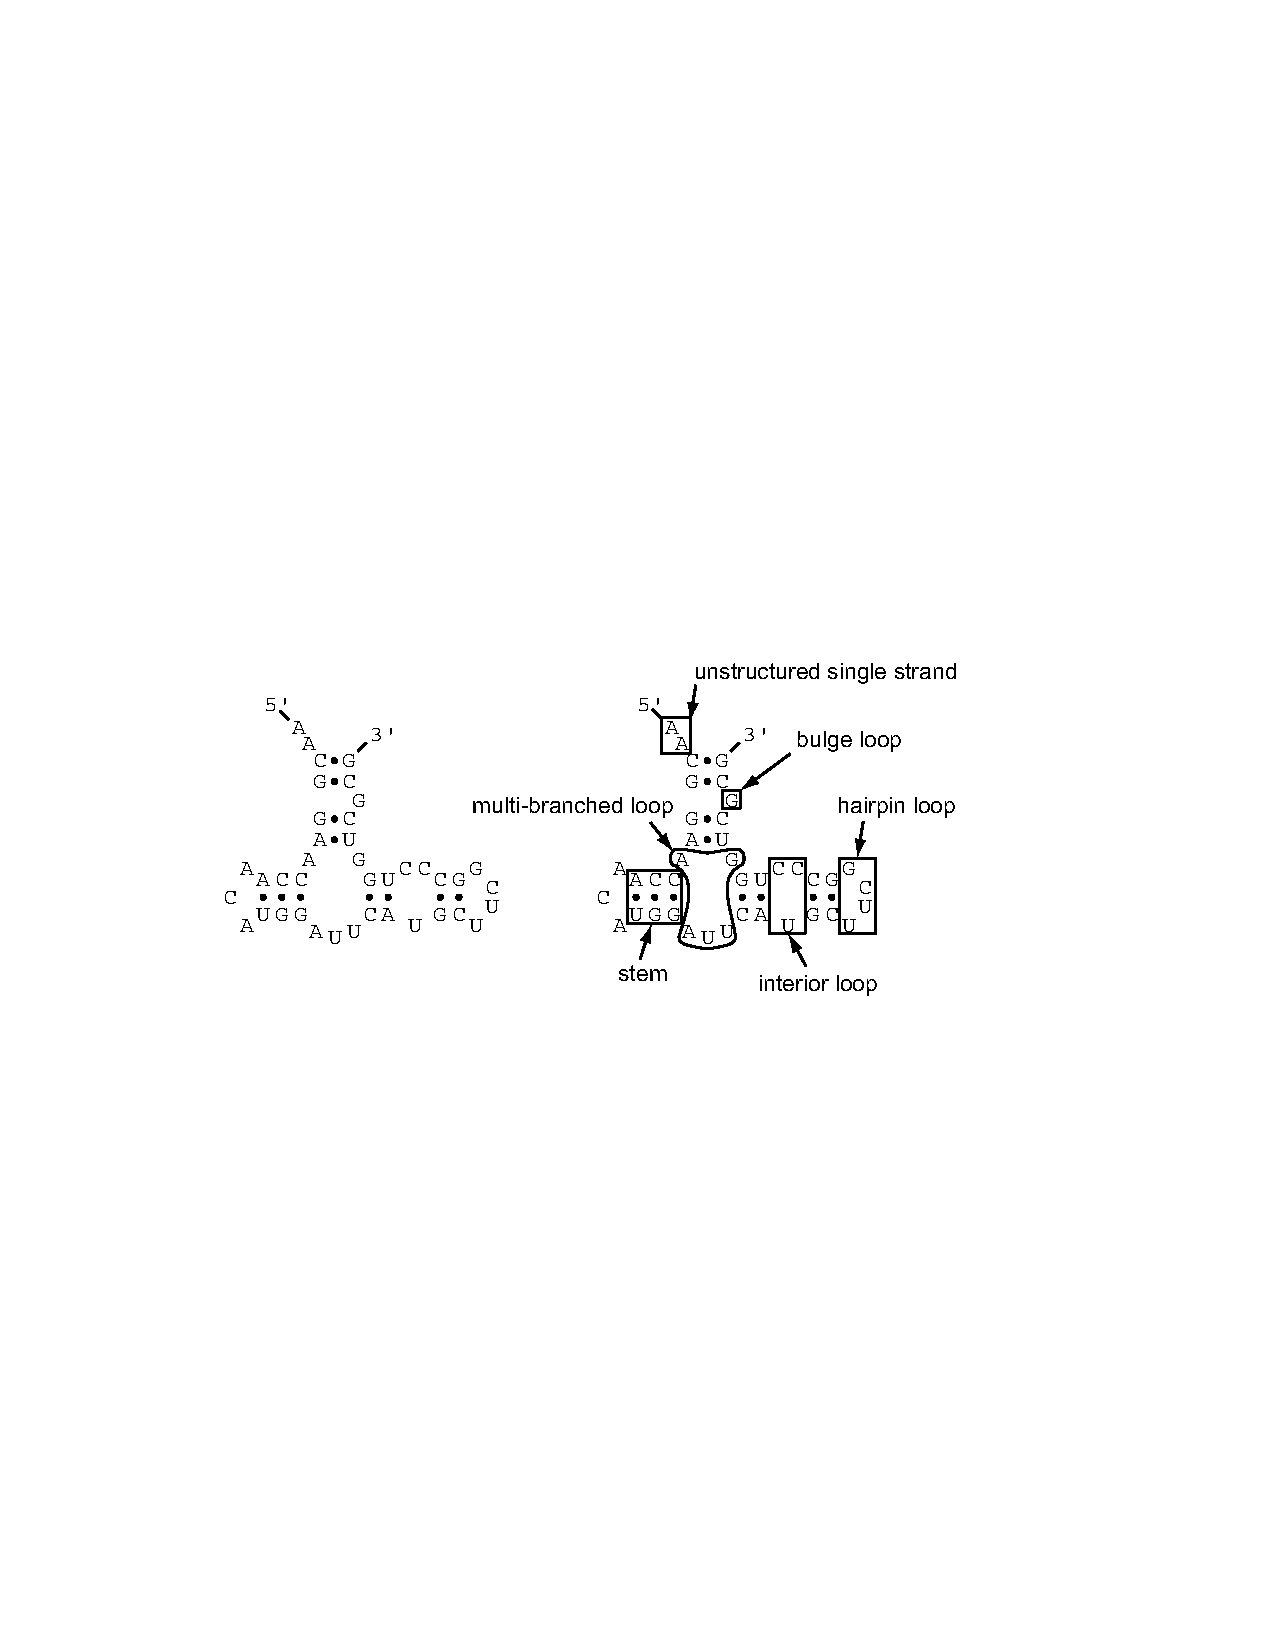
\includegraphics[scale=0.8]{Figures/rna_elements}
\end{center}
\begin{center}
\begin{BVerbatim}
  ::((((,<<<___>>>,,,<<-<<____>>-->>,))-))
  AACGGAACCAACAUGGAUUCAUGCUUCGGCCCUGGUCGCG
\end{BVerbatim}
\end{center}

\subsubsection{Full (output) WUSS notation}

In detail, symbols used by WUSS notation in \emph{output} structure
annotation strings are as follows:

\begin{sreitems}{\textbf{Bulge, interior loops}}
\item[\textbf{Base pairs}]
  Base pairs are annotated by nested matching pairs of symbols
  \verb+<>+, \verb+()+, \verb+[]+, or \verb+{}+.
  The different symbols indicate the ``depth'' of the
  helix in the RNA structure as follows:
  \verb+<>+ are used for simple terminal stems; 
  \verb+()+ are used for ``internal'' helices enclosing a multifurcation of
  all terminal stems; \verb+[]+ are used for internal helices 
  enclosing a multifurcation that includes at least one annotated
  \verb+()+ stem already; and \verb+{}+ are used for all internal
  helices enclosing deeper multifurcations.
   
\item[\textbf{Hairpin loops}]
  Hairpin loop residues are indicated by underscores, \verb+_+.
  Simple stem loops stand out as, e.g.\ \verb+<<<<____>>>>+.

\item[\textbf{Bulge, interior loops}]
  Bulge and interior loop residues are indicated by dashes, \verb+-+.
  
\item[\textbf{Multifurcation loops}]
  Multifurcation loop residues are indicated by commas, \verb+,+.
  The mnemonic is ``stem 1, stem2'', e.g.\ \verb+<<<___>>>,,<<<___>>>+.

\item[\textbf{External residues}]
  Unstructured single stranded residues completely outside the
  structure (unenclosed by any base pairs) are annotated by
  colons, \verb+:+.

\item[\textbf{Insertions}]
  Insertions relative to a known structure are indicated by periods,
  \verb+.+. Regions where local structural alignment was invoked,
  leaving regions of both target and query sequence unaligned,
  are indicated by tildes, \verb+~+. These symbols only appear in
  alignments of a known (query) structure annotation to a target
  sequence of unknown structure.

\item[\textbf{Pseudoknots}]
  WUSS notation allows pseudoknots to be annotated as pairs of
  upper case/lower case letters: for example,
  \verb+<<<<_AAAA____>>>>aaaa+ annotates a simple pseudoknot;
  additional pseudoknotted stems could be annotated by \verb+Bb+,
  \verb+Cc+, etc. \software{infernal} cannot handle pseudoknots, however;
  pseudoknot notation never appears in \software{infernal} output; it
  is accepted in input files, but ignored.
\end{sreitems}

An example of WUSS notation for a complicated structure
(\emph{E. coli} RNase P) is shown in Figure~\ref{fig:RNaseP}.  An
example of WUSS notation for a local \software{infernal} alignment of
\emph{B. subtilis} RNase P to \emph{E. coli} RNase P, illustrating the
use of local alignment annotation symbols, is in
Figure~\ref{fig:bsu-alignment}.

\begin{figure}[tp]
\begin{center}
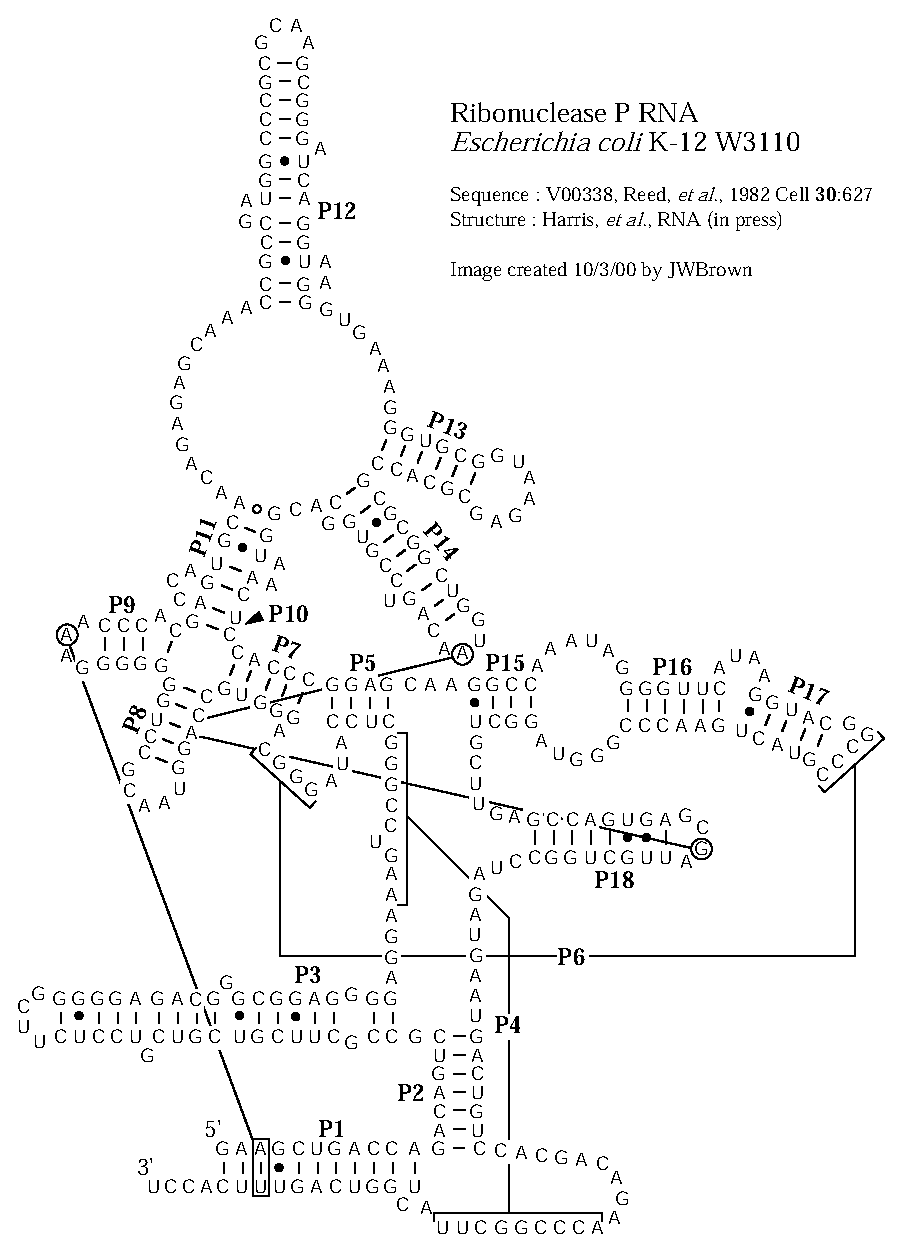
\includegraphics[scale=0.6]{Figures/rnaseP-ecoli}
\end{center}        
\begin{center}
{\scriptsize
\begin{BVerbatim}
           {{{{{{{{{{{{{{{{{{,<<<<<<<<<<<<<-<<<<<____>>>>>>>>>->>>>>>>>
         1 GAAGCUGACCAGACAGUCGCCGCUUCGUCGUCGUCCUCUUCGGGGGAGACGGGCGGAGGG 60      

           >,,,,,,,,,,,,,[[[[--------[[[[[<<<<<_____>>>>><<<<____>>>->(
        61 GAGGAAAGUCCGGGCUCCAUAGGGCAGGGUGCCAGGUAACGCCUGGGGGGGAAACCCACG 120     

           (---(((((,,,,,,,,,,,,<<<<<--<<<<<<<<____>>>>>->>>>>>-->>,,,,
       121 ACCAGUGCAACAGAGAGCAAACCGCCGAUGGCCCGCGCAAGCGGGAUCAGGUAAGGGUGA 180     

           ,,,<<<<<<_______>>>>>><<<<<<<<<____>>>->>>>>->,,)))--))))]]]
       181 AAGGGUGCGGUAAGAGCGCACCGCGCGGCUGGUAACAGUCCGUGGCACGGUAAACUCCAC 240     

           ]]]]]],,,<<<<------<<<<<<----<<<<<_____>>>>>>>>>>>----->>>>,
       241 CCGGAGCAAGGCCAAAUAGGGGUUCAUAAGGUACGGCCCGUACUGAACCCGGGUAGGCUG 300     

           ,,,,,<<<<<<<<____>>>>>>>>,,,,,,,,,,}}}}}}}------------------
       301 CUUGAGCCAGUGAGCGAUUGCUGGCCUAGAUGAAUGACUGUCCACGACAGAACCCGGCUU 360     

           -}-}}}}}}}}}}::::
       361 AUCGGUCAGUUUCACCU 377     
\end{BVerbatim} 
}
\end{center}
\caption{\small \textbf{Example of WUSS notation.} Top: Secondary
structure of \emph{E. coli} RNase P, from Jim Brown's RNase P database
\cite{Brown99}. Bottom: WUSS notation for the same structure,
annotating the \emph{E. coli} RNase P sequence. The P4 and P6
pseudoknots are not annotated in this example.}
\label{fig:RNaseP}
\end{figure}

\begin{figure}[tp]
\begin{center}
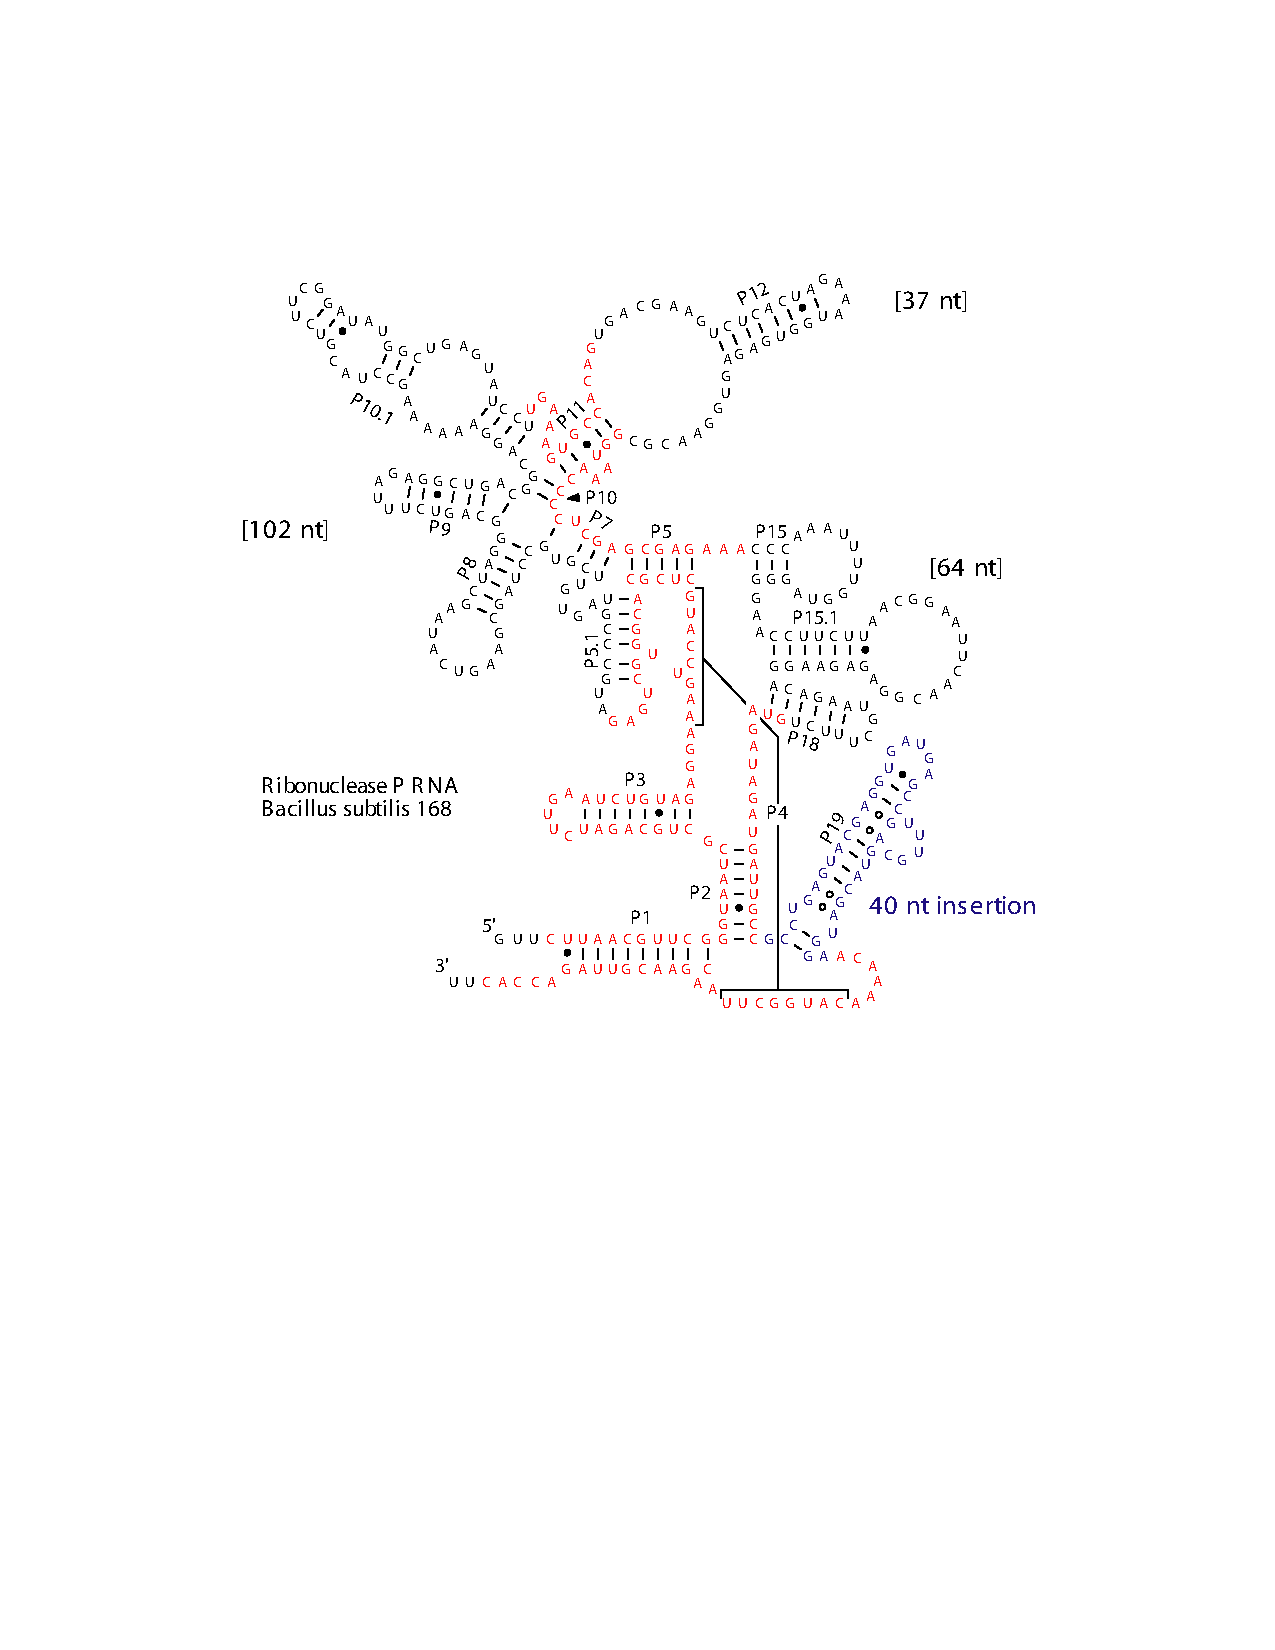
\includegraphics[scale=0.6]{Figures/rnaseP-bsu-alignment}
\end{center}
\begin{center}
{\scriptsize
\begin{BVerbatim}
hit 0   :      4    399    52.56 bits
           {{{{{{{{{{{{{{{{{{,<<<<<<<<<<<<<-<<<<<____>>>>>>>>>->>>>>>>>
         1 ggAGuggGgcaGgCaguCGCugcuucggccuuGuucaguuaacugaaaaggAccgaagga 60      
           +: :::G::C:GG:A:UCGCU+C::::            U+            ::::G+A
         4 CUUAACGUUCGGGUAAUCGCUGCAGAUC-----------UUG----------AAUCUGUA 42      

           >,,,,,,,,,,,,,[[[.[--------[[[[[~~~~~~~((---(((((,,,,~~~~~~)
        61 GAGGAAAGUCCGGGCUC.CACAGGGCAgGGUG*[ 29]*GGAAAGUGCCACAG*[96]*G 229     
           GAGGAAAGUCC  GCUC C  A GG   :G G       :GAAAGUGCCACAG      G
        43 GAGGAAAGUCCAUGCUCgC--ACGGUGCUGAG*[102]*UGAAAGUGCCACAG*[37]*G 226     

           ))--))))]]]]]].]]],,,~~~~~~,,,,,,,,,,}}}}}}}--..............
       230 GUAAACCCCACCcG.GAGCAA*[77]*CuAGAUGAAUGacuGcCCA.............. 344     
           GUAAACC:C C: G GAG AA       UAGAU++AUGA:U:CC                
       227 GUAAACCCCUCGAGcGAGAAA*[64]*GUAGAUAGAUGAUUGCC--gccugaguacgagg 342     

           ..........................-----------------}-}}}}}}}}}}::::
       345 ..........................CGACAGAACCCGGCUUAuagcCccaCUccucuu 377     
                                       ACA AAC  GGCUUA:AG::C::: :+ C  
       343 ugaugagccguuugcaguacgaugga--ACAAAACAUGGCUUACAGAACGUUAGACCAC 399     
\end{BVerbatim}
}
\end{center}
\caption{\small \textbf{Local alignment annotation example.} Top:
Secondary
structure of \emph{B. subtilis} RNase P, from Jim Brown's RNase P
database \cite{Brown99}. Residues in red are those that \software{infernal} aligns
to a CM of \emph{E. coli} type RNase P's. The local structural
alignment is in four pieces; three regions of the
structure (102, 37, and 64 nt long) are skipped over. One additional
stem is treated as a 40 nt insertion. Bottom: the \software{infernal}
output, showing the \emph{E. coli} query structure aligned to the
\emph{B. subtilis} sequence.}
\label{fig:bsu-alignment}
\end{figure}

\subsubsection{Shorthand (input) WUSS notation}

While WUSS notation makes it easier to visually interpret
\software{infernal} \emph{output} structural annotation, it would be
painful to be required to \emph{input} all structures in full WUSS
notation. Therefore when \software{infernal} reads input secondary
structure annotation, it uses simpler rules:

\begin{sreitems}{\textbf{Single stranded residues}}
\item [\textbf{Base pairs}]
  Any matching nested pair of \verb+()+, \verb+()+, \verb+[]+, \verb+{}+
  symbols indicates a base pair; the exact choice of symbol has no
  meaning, so long as the left and right partners match up.

\item [\textbf{Single stranded residues}]
  All other symbols \verb+_-,:.~+ 
  indicate single stranded residues.
  The choice of symbol has no special meaning.
  Annotated pseudoknots (nested matched pairs of upper/lower case
  alphabetic characters) are also interpreted as single
  stranded residue in \software{infernal} input.
\end{sreitems}

Thus, for instance, \verb+<<<<....>>>>+ and \verb+((((____))))+ and
\verb+<(<(._._)>)>+ all indicate a four base stem with a four base
loop (the last example is legal but weird). 

Remember that the key property of canonical (nonpseudoknotted) RNA
secondary structure is that the pairs are \emph{nested}.
\verb+((<<....))>>+ is not a legal annotation string: the pair symbols
don't match up properly. \software{infernal} will reject such an
annotation and report an input format error, suspecting a problem with
your annotation.  If you want to annotate pseudoknots, WUSS notation
allows alphabetic symbols Aa, Bb, etc.\, see above; but remember that
\software{infernal} ignores pseudoknotted stems and treats them as
single stranded residues.

Because many other RNA secondary structure analysis programs use a
simple bracket notation for annotating structure,
\software{infernal}'s ability to input this format makes it easier to
use data generated by other RNA software packages. Conversely,
converting \software{infernal} output WUSS notation to simple bracket
notation is a matter of a simple Perl or sed script, substituting the
symbols appropriately.

\subsection{Multiple alignments: Stockholm format}
\label{pg:stockholm}

The Pfam consortium developed an annotated alignment format called
``Stockholm format'', and this format has been adopted as the standard
alignment format in \software{hmmer} and \software{infernal}, and by
the Rfam consortium. The reasons for inventing a new alignment format
were two-fold. First, there really is no standard accepted format for
multiple sequence alignment files, so we don't feel guilty about
inventing a new one. Second, the formats of popular multiple alignment
software (e.g. CLUSTAL, GCG MSF, PHYLIP) do not support rich
documentation and markup of the alignment.  Stockholm format was
developed to support extensible markup of multiple sequence
alignments, and we use this capability extensively in both RNA work
(with structural markup) and the Pfam database (with extensive use of
both annotation and markup).

\subsubsection{A minimal Stockholm file}
\begin{sreoutput}
# STOCKHOLM 1.0

seq1  ACDEF...GHIKL
seq2  ACDEF...GHIKL
seq3  ...EFMNRGHIKL

seq1  MNPQTVWY
seq2  MNPQTVWY
seq3  MNPQT...
\end{sreoutput}

The simplest Stockholm file is pretty intuitive, easily generated in a
text editor. It is usually easy to convert alignment formats into a
``least common denominator'' Stockholm format. For instance, SELEX,
GCG's MSF format, and the output of the CLUSTAL multiple alignment
programs are all similar interleaved formats.

The first line in the file must be \verb+# STOCKHOLM 1.x+, where
\verb+x+ is a minor version number for the format specification (and
which currently has no effect on my parsers, other than identifying
the file as Stockholm format). This line allows a parser to instantly
identify the file format.

In the alignment, each line contains a name, followed by the aligned
sequence. A dash or period denotes a gap. If the alignment is too long
to fit on one line, the alignment may be split into multiple blocks,
with blocks separated by blank lines. The number of sequences, their
order, and their names must be the same in every block. Within a given
block, each (sub)sequence (and any associated \verb+#=GR+ and
\verb+#=GC+ markup, see below) is of equal length, called the
\textit{block length}. Block lengths may differ from block to block;
the block length must be at least one residue, and there is no
maximum.  

The sequence names must be unique. (They are used to associate markup
tags with the sequences.)

Other blank lines are ignored. You can add comments to the file on
lines starting with a \verb+#+.

All other annotation is added using a tag/value comment style. The
tag/value format is inherently extensible, and readily made
backwards-compatible; unrecognized tags will simply be ignored. Extra
annotation includes consensus and individual RNA or protein secondary
structure, sequence weights, a reference coordinate system for the
columns, and database source information including name, accession
number, and coordinates (for subsequences extracted from a longer
source sequence) See below for details.

\subsubsection{Syntax of Stockholm markup}

There are four types of Stockholm markup annotation, for per-file,
per-sequence, per-column, and per-residue annotation:

\begin{sreitems}{\prog{\#=GR <seqname> <tag> <s>}}
\item [\emprog{\#=GF <tag> <s>}]
	Per-file annotation. \prog{<s>} is a free format text line
	of annotation type \prog{<tag>}. For example, \prog{\#=GF DATE
	April 1, 2000}. Can occur anywhere in the file, but usually
	all the \prog{\#=GF} markups occur in a header.

\item [\emprog{\#=GS <seqname> <tag> <s>}]
	Per-sequence annotation. \prog{<s>} is a free format text line
	of annotation type \prog{tag} associated with the sequence
	named \prog{<seqname>}. For example, \prog{\#=GS seq1
	SPECIES\_SOURCE Caenorhabditis elegans}. Can occur anywhere
	in the file, but in single-block formats (e.g. the Pfam
	distribution) will typically follow on the line after the
	sequence itself, and in multi-block formats (e.g. HMMER
	output), will typically occur in the header preceding the
	alignment but following the \prog{\#=GF} annotation.

\item [\emprog{\#=GC <tag> <s>}]
	Per-column annotation. \prog{<s>} is an aligned text line
	of annotation type \prog{<tag>}.
        \verb+#=GC+ lines are
	associated with a sequence alignment block; \prog{<s>}
	is aligned to the residues in the alignment block, and has
	the same length as the rest of the block.
	Typically \verb+#=GC+ lines are placed at the end of each block.

\item [\emprog{\#=GR <seqname> <tag> <s>}]
	Per-residue annotation. \prog{<s>} is an aligned text line
	of annotation type \prog{<tag>}, associated with the sequence
	named \prog{<seqname>}. 
	\verb+#=GR+ lines are 
	associated with one sequence in a sequence alignment block; 
	\prog{<s>}
	is aligned to the residues in that sequence, and has
	the same length as the rest of the block.
	Typically
        \verb+#=GR+ lines are placed immediately following the
	aligned	sequence they annotate.
\end{sreitems}

\subsubsection{Semantics of Stockholm markup}

Any Stockholm parser will accept syntactically correct files, but is
not obligated to do anything with the markup lines. It is up to the
application whether it will attempt to interpret the meaning (the
semantics) of the markup in a useful way. At the two extremes are the
Belvu alignment viewer and the HMMER profile hidden Markov model
software package.

Belvu simply reads Stockholm markup and displays it, without trying to
interpret it at all. The tag types (\prog{\#=GF}, etc.) are sufficient
to tell Belvu how to display the markup: whether it is attached to the
whole file, sequences, columns, or residues.

\software{hmmer} and \software{infernal} use Stockholm markup to pick
up a variety of information from the multiple alignment files. The
Pfam and Rfam consortiums therefore agree on additional syntax for
certain tag types, so software can parse some markups for useful (or
necessary) information. This additional syntax is imposed by Pfam,
\software{hmmer}, \software{infernal}, and other software of mine, not
by Stockholm format per se. You can think of Stockholm as akin to XML,
and what my software reads as akin to an XML DTD, if you're into that
sort of structured data format lingo.

The Stockholm markup tags that are parsed semantically by my software
are as follows:

\subsubsection{Recognized \#=GF annotations}
\begin{sreitems}{\emprog{AU  <s>}}
\item [\emprog{ID  <s>}] 
	Identifier. \emprog{<s>} is a name for the alignment;
	e.g. ``RNaseP. Mandatory, if the file is an alignment
        database used as input for \prog{cmbuild}, because 
        each CM must get a unique name. One word. Unique in file.

\item [\emprog{AC  <s>}]
	Accession. \emprog{<s>} is a unique accession number for the
	alignment; e.g. 
	``PF00001''. Used by the Rfam database, for instance. 
	Often a alphabetical prefix indicating the database
	(e.g. ``RF'') followed by a unique numerical accession.
	One word. Unique in file. 
	
\item [\emprog{DE  <s>}]
	Description. \emprog{<s>} is a free format line giving
	a description of the alignment; e.g.
	``Ribonuclease P RNA''. One line. Unique in file.

\item [\emprog{AU  <s>}]
	Author. \emprog{<s>} is a free format line listing the 
	authors responsible for an alignment; e.g. 
	``Bateman A''. One line. Unique in file.
\end{sreitems}

\subsubsection{Recognized \#=GS annotations}

\begin{sreitems}{\emprog{WT  <f>}}
\item [\emprog{WT  <f>}]
	Sequence weight. \emprog{<f>} is a positive real number giving the
	relative weight for a sequence, usually used to compensate
	for biased representation by downweighting similar sequences.	
	Usually the weights average 1.0 (e.g. the weights sum to
	the number of sequences in the alignment) but this is not
	required. Either every sequence must have a weight annotated, 
	or none	of them can.  

\item [\emprog{AC  <s>}]
	Accession. \emprog{<s>} is a database accession number for 
	this sequence. (Compare the \prog{\#=GF AC} markup, which gives
	an accession for the whole alignment.) One word. 
	
\item [\emprog{DE  <s>}]
	Description. \emprog{<s>} is one line giving a description for
	this sequence. (Compare the \prog{\#=GF DE} markup, which gives
	a description for the whole alignment.)
\end{sreitems}

\subsubsection{Recognized \#=GC annotations}

\begin{sreitems}{\emprog{SS\_cons}}
\item [\emprog{RF}]
	Reference line. Any character is accepted as a markup for a
	column. The intent is to allow labeling the columns with some
	sort of mark. \prog{cmbuild} uses this annotation to 
        determine which columns are consensus versus insertion;
        insertion columns are annotated by a gap symbol, and consensus
        columns by any non-gap symbol.
	
\item [\emprog{SS\_cons}]
	Secondary structure consensus. 
        When this line is generated by \software{infernal}, it is generated in full WUSS
        notation.
	When it is read by \prog{cmbuild}, it is interpreted more
        loosely, in shorthand (input) WUSS notation:
	pairs of symbols \verb+<>+, \verb+()+, \verb+[]+, or \verb+[]+ mark
	consensus base pairs, and symbols \verb+:_-,.~+ mark single
        stranded columns. 
\end{sreitems}

\subsubsection{Recognized \#=GR annotations}

\begin{sreitems}{\emprog{SS}}
\item [\emprog{SS}]
	Secondary structure for this sequence. See \prog{\#=GC
        SS\_cons} above. 
\end{sreitems}

\subsection{Sequence files: FASTA format}

FASTA is probably the simplest of formats for unaligned sequences.
FASTA files are easily created in a text editor.  Each sequence is
preceded by a line starting with \verb+>+. The first word on this line
is the name of the sequence. The rest of the line is a description of
the sequence (free format). The remaining lines contain the sequence
itself. You can put as many letters on a sequence line as you want.
For example:

\begin{sreoutput}
>seq1 This is the description of my first sequence.
AGTACGTAGTAGCTGCTGCTACGTGCGCTAGCTAGTACGTCA CGACGTAGATGCTAGCTGACTCGATGC
>seq2 This is a description of my second sequence.
CGATCGATCGTACGTCGACTGATCGTAGCTACGTCGTACGTAG CATCGTCAGTTACTGCATGCTCG
CATCAGGCATGCTGCTGACTGATCGTACG
\end{sreoutput}

For better or worse, FASTA is not a documented standard. Minor (and
major) variants are in widespread use in the bioinformatics community,
all of which are called ``FASTA format''. My software attempts to
cater to all of them, and is tolerant of common deviations in FASTA
format. Certainly anything that is accepted by the database formatting
programs in NCBI BLAST or WU-BLAST (e.g. setdb, pressdb, xdformat)
will also be accepted by my software. Blank lines in a FASTA file are
ignored, and so are spaces or other gap symbols (dashes, underscores,
periods) in a sequence. Other non-amino or non-nucleic acid symbols in
the sequence are also silently ignored, mostly because some people
seem to think that ``*'' or ``.'' should be added to protein sequences
to (redundantly) indicate the end of the sequence. The parser will
also accept unlimited line lengths, which allows it to accomodate the
enormous description lines in the NCBI NR databases.

(On the other hand, any FASTA files \emph{generated} by my software
adhere closely to community standards, and should be usable by other
software packages (BLAST, FASTA, etc.) that are more picky about
parsing their input files. That means you can run a sloppy FASTA file
thru the \prog{sreformat} utility program to clean it up.)

Partly because of this tolerance, the software may have a difficult
time dealing with files that are \textit{not} in FASTA format,
especially if you're relying on file format autodetection (the
``Babelfish'').  Some (now mercifully uncommon) file formats are so
similar to FASTA format that they be erroneously called FASTA by the
Babelfish and then quietly and lethally misparsed. An example is the
old NBRF file format. If you're afraid of this, you can use the
\prog{--informat fasta} option to bypass the Babelfish and improve
robustness. However, it is still possible to construct files
perversely similar to FASTA that will still confuse the parser.  (The
gist of these caveats applies to all formats, not just FASTA.)

\subsection{CM file format}

The default CM file format is a simple, extensible tag-value format.
The format being used right now is tentative and likely to
change. Therefore, it is not currently documented here. If you
absolutely need to interpret it, see the file \verb+cm_io.c+ in the
source code.

\subsection{Null model file format}

The Infernal source distribution includes an example prior file, 
\prog{rna.null}. This null model is identical to the hardcoded default
prior used by Infernal, all four RNA nucleotides are equiprobable in
the null, background model. 

A null model file must contain exactly four non-comment lines. A
comment line begins with a ``\# ``, that is a \# followed by a single
space. Each of the four non-comment lines must contain a single floating point
number, the four of which sum to 1.0. The first non-comment line is interpreted as
the background probability of an ``A'' residue, the second, third, and
fourth non-comment lines are interpreted as the background
probabilities of a ``C'', ``G'' and ``U'' respectively. 




